%second chapter of your thesis
\chapter{Literatuurstudie}
%intro
\section{\acrfull{vlc}}
	%RF bandwidths are failing to meet requirements, VLC is promising alternatives
	%korte intro
	De \acrfull{led} is een technologie dat gebruikt kan worden voor verlichting als communicatie. Hierdoor is het geschikt voor optische draadloze communicatie in de vrije ruimte. \gls{vlc} is een technologie dat hier op bouwt en veel verwachting heeft naar toekomstige applicaties toe. 
\section{\acrfull{vlp}}
	Naast communicatie is lokalisatie nog een belangrijke toepassing met een groot potentieel. Op plekken waar traditionele lokalisatiemethoden zoals GPS falen, zoals indoor scenario's, is men op zoek naar een technologie die wel kan voldoen aan de voorschriften. \acrfull{vlp} is naast o.a. \acrfull{uwb}, \acrfull{rfid}, Wi-Fi en fingerprint een uitdager om deze rol in te vullen. Het nadeel van deze laatste technologie\"en is dat er nood is aan het installeren van een extra \acrfull{ap} en apparatuur. Dit leidt tot stijgende kosten voor het installeren, gebruik en onderhoud.
	\gls{vlp} is veel belovend juist omdat het deze extra kosten kan vermijden door de duale rol van de apparatuur. De \glspl{led} zorgen voor zowel verlichting als lokalisatie in dezelfde behuizing, door slechts één installatie en heeft dezelfde noden als gewone verlichting. In komende paragrafen leggen we verschillende onderdelen en technieken van \gls{vlp} uit.
	\subsection{Indoor Positioning Techniques}
	\gls{vlc}-based-\gls{ips} kan op verscheidene manieren uitgevoerd worden. In de paragrafen hieronder bespreken we hoe de verschillende technieken ingevuld kunnen worden. We bespreken onder andere \gls{led} technologie, modulatiemethodes, type ontvangers en classificatie van \gls{vlc}-based-\gls{ips} op basis van 3 sleuteleigenschappen.
	
		\subsubsection{\gls{led} Technologie}
		Door het lage vermogensverbruik en de lange levensduur is \gls{led} een veel gebruikt middel om verlichting van ruimtes te bereiken. Er zijn twee veelgebruikte \gls{led}-technologie\"en om wit licht te produceren: 
		
			\begin{itemize}
				\item \textbf{White \glspl{led}:} Bij dit ontwerp cre\"ert men wit licht door een gele fosfor over een blauwe \gls{led} te plaatsen. De combinatie van zowel de gele fosfor als het blauwe uitgestraalde licht zorgt dat ons oog de stralen als wit licht interpreteert. De eenvoud laat toe om de prijs en de complexiteit laag te houden, waardoor dit de meest gekozen techniek is.
				
				\item \textbf{RGB-\glspl{led}:} Door de combinatie van de kleuren rood, groen en blauw is het ook mogelijk om een wit licht te cre\"eren. Deze optie vraagt wel om twee extra \glspl{led} waardoor de kostprijs stijgt. Het gebruik van de RGB-\glspl{led} heeft wel het voordeel dat er aan \gls{csk} kan gedaan worden. Deze methode heeft dus een bredere functionaliteit.
			\end{itemize}
		
		\subsubsection{Modulatiemethode}
		Doordat de \glspl{led} voor zowel verlichting als communicatie dienen is van uiterst belang dat voorzieningen voor het ene, het andere niet in gedrang brengen. De gekozen modulatiemethode voor communicatie moet dus ondersteuning bieden zodat de werking van de verlichting normaal kan blijven verlopen. Om hier aan te voldoen moet er dus ondersteuning zijn voor dimming en flicker controle.
			\begin{itemize}
				\item \textbf{\acrfull{ook}:} \gls{ook} is de simpelste vorm van \acrfull{ask} modulatie waarbij de \gls{led} aan en uit wordt gezet. De eenvoudige implementatie is de reden waarom de techniek wijd gebruikt wordt in de draadloze communicatie. Er kan een onderscheid gemaakt worden tussen \acrfull{nrz} \gls{ook} en \acrfull{rz}\gls{ook}. Bij \gls{rz}\gls{ook} zal het signaal terug naar 0 gaan achter elk uitgezonden symbool. Dit zorgt ervoor dat de grote van de bandbreedte verdubbeld terwijl de data rate hetzelfde blijft. Echter biedt \gls{ook} geen ondersteuning voor zowel dimming of flicker controle.
				
				\item \textbf{\acrfull{ppm}:} \gls{ppm} is een modulatiemethode waarbij bits gecodeerd worden door een puls op een bepaalde plaats of tijdstip uit te zenden. De symboolduur is onderverdeeld in T verschillende tijdslots en de positie van de puls bepaalt het verzonden symbool. Dit is ook een eenvoudige versie waar veel varianten op bestaan. Zo zijn er \acrfull{vppm}, \acrfull{oppm}, \acrfull{mppm} en nog veel meer. Elk met zijn voordelen en nadelen die afgewogen moeten worden bij het maken van een keuze. 
				
				\item \textbf{\acrfull{ofdm}:} \gls{ofdm} kan gebruikt worden om in het kader van VLC \acrfull{isi} te verminderen en het gebruik van bandbreedte te verbreden. De methode staat toe om data te encoderen op meerdere carrierfrequenties. Deze carriers overlappen elkaar op het frequentiespectrum en voor demodulatie worden er Fast Fourier Transformatie algoritmes gebruikt.
				
				\item \textbf{\acrfull{csk}:} In \gls{csk} varieert de kleuren rood, groen en blauw in een \gls{led} om een signaal te moduleren. Dit maakt het geschikter voor VLC dan gebruikelijke technieken doordat men met een hogere bandbreedte kan werken, en makkelijker dimming en flicker controle kan implementeren.
			\end{itemize}
		
		\subsubsection{Type ontvanger}
		De ontvanger is een belangrijk onderdeel van het positieneersysteem. Het ontvangen van data zoals ID, positie, signaalsterkte en \gls{toa} zijn afhankelijk van het type ontvanger. Ook de data rate is een belangrijke factor die meespeelt in de keuze. We kunnen de types ontvanger onderverdelen in twee categorie\"en: De photodiode en Image Sensors.
			\begin{itemize}
				\item \textbf{\gls{pd}:} De \gls{pd} bestaat uit halfgeleidermateriaal dat invallende fotonen omzet in een elektrische stroom. Deze kunnen in verschillende formaten voorkomen en gevoelig zijn voor bepaalde delen van het optisch spectrum door middel van optische filters. Door de snelle responsie is de \gls{pd} geschikt voor \gls{rss}, \gls{toa} en \gls{tdoa} algoritmes.
				
				\item \textbf{Image Sensors:}  Vergeleken met de \gls{pd} is de Image Sensor een goedkopere optie. De Image Sensor of imager zet lichtgolven om in elektrische stroom.
				\todo{verschil PD en image sensors uitleggen, nog op te zoeken}
			\end{itemize}
	\subsection{Classificatie}
	% classificatie van VLC-based-IPS op 3 keyeigenschappen
		\subsubsection{Wiskundige methode}
		
			\begin{itemize}
				\item Proximity
				\item Triangulation
					\begin{itemize}
						\item \acrfull{aoa}
						\item \acrfull{toa}
						\item \acrfull{rss}
					\end{itemize}
				\item Fingerprint
					\begin{itemize}
						\item Map-Based fingerprint
						\item Online stage/runtime stage
					\end{itemize}
			\end{itemize}
		\subsubsection{Sensor assisted methode}
		\subsubsection{Optimization methode}
		
\newpage

\section{\gls{ann}}
\gls{ann} is een term dat gebruikt wordt om een algoritme te omschrijven dat lijkt op maar niet hetzelfde is als een biologisch neuraal netwerk in de hersens van dieren. Deze systemen zijn in staat om een bepaalde taak te leren, en zichzelf te verbeteren. In de meeste gevallen worden er zelf geen richtlijnen of omschrijving meegegeven. Het systeem ontdekt zelf hoe deze regels in elkaar zitten. Een bekend voorbeeld is het herkennen van de cijfers 0 tot 9. Hierin wordt er niet aan het systeem verteld dat het cijfer 8 uit twee cirkels bestaat die verticaal tegen elkaar aansluiten. Het algoritme zal dit gaandeweg ontdekken met behulp van de vele voorbeelden waar het gebruik van kan maken. Met behulp van veel data kan een algoritme zichzelf verfijnen en nauwkeuriger bepaalde cijfers herkennen.

	\subsection{Structuur van een \gls{nn}}
	Een \gls{ann} is verzameling van nodes die met elkaar verbonden zijn zoals neuronen in de hersens van een mens. Hierbij kan elke neuron een signaal doorgeven naar de volgende neuron waar het signaal verwerkt kan worden en weer doorgegeven kan worden. Hetzelfde principe geldt ook bij \gls{nn} met het verschil dat er meerdere lagen van nodes te onderscheiden zijn. 
	
	\begin{figure}
	    \centering
		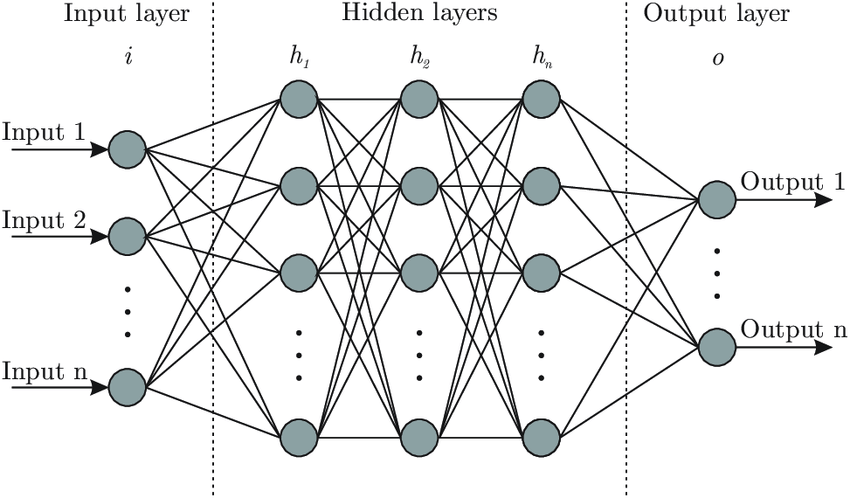
\includegraphics[width=140mm]{afbeeldingen/neuralNetwork2.PNG}
		\caption{Structuur van een Neuraal Netwerk}
		\label{fig:neuralNetworkStructuur}
	\end{figure}

		\subsubsection{Lagen}
		Er zijn drie soorten lagen te onderscheiden: een Input Layer, Hidden Layers en een Output Layer. Elke laag is verbonden met de volgende laag door middel van de connecties of \textit{edges} tussen de verschillende nodes. In figuur \ref{fig:neuralNetworkStructuur} is de algemene vorm te vinden van een \gls{nn}.
		\begin{itemize}
			\item \textbf{Input Layer:} De eerste laag van elk \gls{nn} is de Input Layer. Deze bestaat uit een aantal inputnodes. Elke inputnode krijgt de ruwe data binnen waar er een operatie op uitgevoerd wordt en vervolgens bepaalde parameters doorgeeft aan de volgende laag. 
			\item \textbf{Hidden Layers:}  Na de inputlaag komen een aantal Hidden Layers. Het aantal Hidden Layers en de hoeveelheid nodes binnen \'e\'en Hidden Layer kan vari\"eren van applicatie tot applicatie en is sterk gerelateerd aan de complexiteit van de toepassing.
			\item \textbf{Output Layer:} Na de Hidden Layers is de laatste laag de Output Layer. Hier worden de laatste operaties uitgevoerd en worden de eindwaarden verkregen.
		\end{itemize}
		
		\subsubsection{Nodes}
		Een node is op zich gebaseerd op zijn biologisch tegenbeeld. Het krijgt een bepaald aantal inputs, verwerkt deze en geeft een bepaald aantal outputs. Deze inputs en outputs worden van node naar node doorgegeven via verbindingen. Elke node heeft met elke node in de volgende laag een connectie. Deze worden \textit{edges} genoemd. Elke edge draagt een bepaald gewicht. Via dit gewicht kan de invloed van de  huidige node versterken of verzwakken in de volgende node.
		
		\subsubsection{Propagation function}
		De mathematische functie die een node gebruikt voor het verwerken van inputs naar outputs heet de propagatie functie.
		In figuur \ref{fig:artificial_neuron} bespreken we de algemene vorm van een neuron. 
		Voor een bepaalde neuron met m+1 inputs $\left(  x_0 t.e.m. x_m \right) $ en bijhorende gewichten $\left(  w_0 t.e.m. w_m \right) $.
		Gebruikelijk wordt $x_0 = +1$ genomen. Hierdoor blijven er maar m echte inputs over waardoor er voor een bepaalde output volgende functie opgesteld kan worden. Hierbij is $\phi$ een van de mogelijke transfer functies die verder besproken zal worden.
		
		
		\begin{equation}
			y_k = \phi \left( \sum_{j=0}^{m}w_{kj}x_j\right) 
		\end{equation}
		
		\begin{figure}
			\centering
			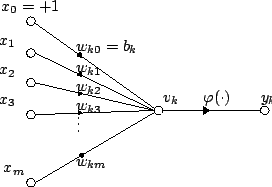
\includegraphics[width=60mm]{afbeeldingen/Artificial_neuron.PNG}
			\caption{Algemene structuur van een node}
			\label{fig:artificial_neuron}
		\end{figure}
		\paragraph{types transfer functies}
		De transfer functie of activatiefunctie van een neuron bevat bepaalde eigenschappen die het volledige netwerk kan verbeteren of versimpelen. Hieronder bespreken we enkele transfer functies.

		\begin{itemize}
			\item \textbf{Stapfunctie:} Hier wordt er gekeken naar de verkregen waarde van de gewogen som u van m+1 inputs. Bedraagt deze waarde minder dan een bepaalde drempel $\theta$, dan wordt de output gelijkgesteld aan nul, bij een hogere waarde dan weer aan 1. Dit is te zien in formule \ref{eq:stapfunctie}. Dit type wordt vooral gebruikt om binaire inputs te verzorgen bij de volgende laag. 
			\begin{equation}
				u =  \left( \sum_{j=0}^{m}w_{kj}x_j\right) 
			\end{equation}
			\begin{equation}\label{eq:stapfunctie}
			y={\begin{cases}1&{\text{als }}u\geq \theta
					   	\\0&{\text{als }}u<\theta \end{cases}}
			\end{equation}
			
			\item \textbf{Lineare Combinaties:} In dit geval is de output niets minder dan de gewogen som plus e
			\item \textbf{Sigmoid:}
			\item \textbf{Rectifier:}
		\end{itemize}
		\paragraph{Leer technieken}
		Om een neuraal netwerk te laten leren zijn er verschillende parkours om te bewandelen de drie belangrijkste methodes om een mathematische functie te verkrijgen worden hieronder opgesomd.
		\begin{itemize}
			\item \textbf{Supervised Learning:} Deze techniek maakt gebruik van gepaarde datasets van inputobjecten en de te verwachten outputobjecten. Het doel is om een mathematische functie te cre\"eren waarbij de gegenereerde outputs zo nauw mogelijk overeenkomen met de gelabelde outputs uit de datasets. De functie kan dan ook gebruikt worden voor nieuwe datasets zonder gelabelde output. Een toepassing van Supervised Learning is bijvoorbeeld het detecteren van spam met een trainingset van al gelabelde e-mails.
			
			\item \textbf{Unsupervised Learning:} Unsupervised learning is een techniek dat gebruik maakt van Hebbian Learning om onbekende patronen te ontdekken in datasets. De twee meestgebruikte methodes onder Unsupervised Learning zijn principal component en cluster analysis. De tweede methode is .../////////
			Een belangrijke toepassing van Unsupervised Learning is het clusteren van gelijkaardige documenten op basis van de inhoud van de tekst.
			% Discovering patterns in unlabeled data Example: cluster similar documents based on the text content
			\item \textbf{Reinforcement Learning:} Deze leertechniek heeft betrekking tot hoe agents acties moeten ondernemen in een omgeving om een bepaald attribuut te maximaliseren. Het verschilt van Supervised en Unsupervised Learning door de onafhankelijkheid van gelabelde outputdatasets en dat minder optimale acties niet manueel gecorrigeerd worden. De techniek heeft als doel om een evenwicht te vinden tussen exploratie van ongekend gebied en exploitatie van de huidige kennis. In figuur \ref{fig:reinforcemntLearning} kan je een eenvoudige routine vinden van Reinforcement Learning-algoritme. Hierbij maakt een agent een bepaalde actie gebaseerd op de staat waar hij in is. Deze actie heeft in een omgeving een zekere invloed die door een Interpreter beoordeeld wordt en een score toekent. De agent kan deze verandering daarna gebruiken om zichzelf te verbeteren en zijn acties aanpassen. 
			\begin{figure}
				\centering
				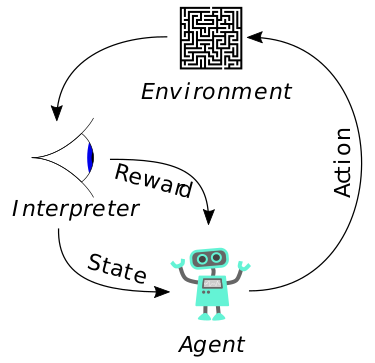
\includegraphics[width=60mm]{afbeeldingen/Reinforcement_learning_diagram.PNG}
				\caption{Routine bij Reinforcement Learning}
				\label{fig:reinforcemntLearning}
			\end{figure}
			Een van de vele mogelijke toepassingen van Reinforcement Learning is het aanleren van schaken door enkel mee te geven of het algoritme gewonnen of verloren heeft. 

		\end{itemize}

\newpage		
\section{Evolutie \gls{sbc}}
Een \gls{sbc} is een volledige computer gemaakt op 1 enkele printplaat. Het bevat onderdelen zoals een microprocessor, geheugen, inputs en outputs. De \gls{sbc} werd ontwikkeld als een voorstel-hulpmiddel bij educatieve doelstellingen of het gebruik als een embedded computer controller. Tegenwoordig zijn ook vele (draagbare) computers ge\"integreerd op \'e\'en printplaat. Het grote verschil met (draagbare) computers is dat er geen nood is aan expansion slots zoals bijvoorbeeld voor RAM-geheugen of een \gls{gpu}.
	\subsection{Geschiedenis}
	De eerste echte SBC was de zogenaamde "dyna-micro"\space uit figuur \ref{fig:eersteSBC} die later de naam "MMD-1" (Mini-Micro Designer 1) kreeg. Dit toestel werd uitgegeven in 1976 en werd populair doordat het werd gepresenteerd in het destijds 'BugBook' als het voorbeeld microprocessor. Een andere vroege \gls{sbc} was de KIM-1 (Keyboard Input Monitor 1) uit hetzelfde jaar. Beide machines werden voor ingenieurs geproduceerd en ontworpen maar vonden een breed publiek onder de hobbyisten waar het heel populair was. Later kwamen nog andere namen zoals de Ferguson Big Board en de Nascom.

	\begin{figure}
		\centering
		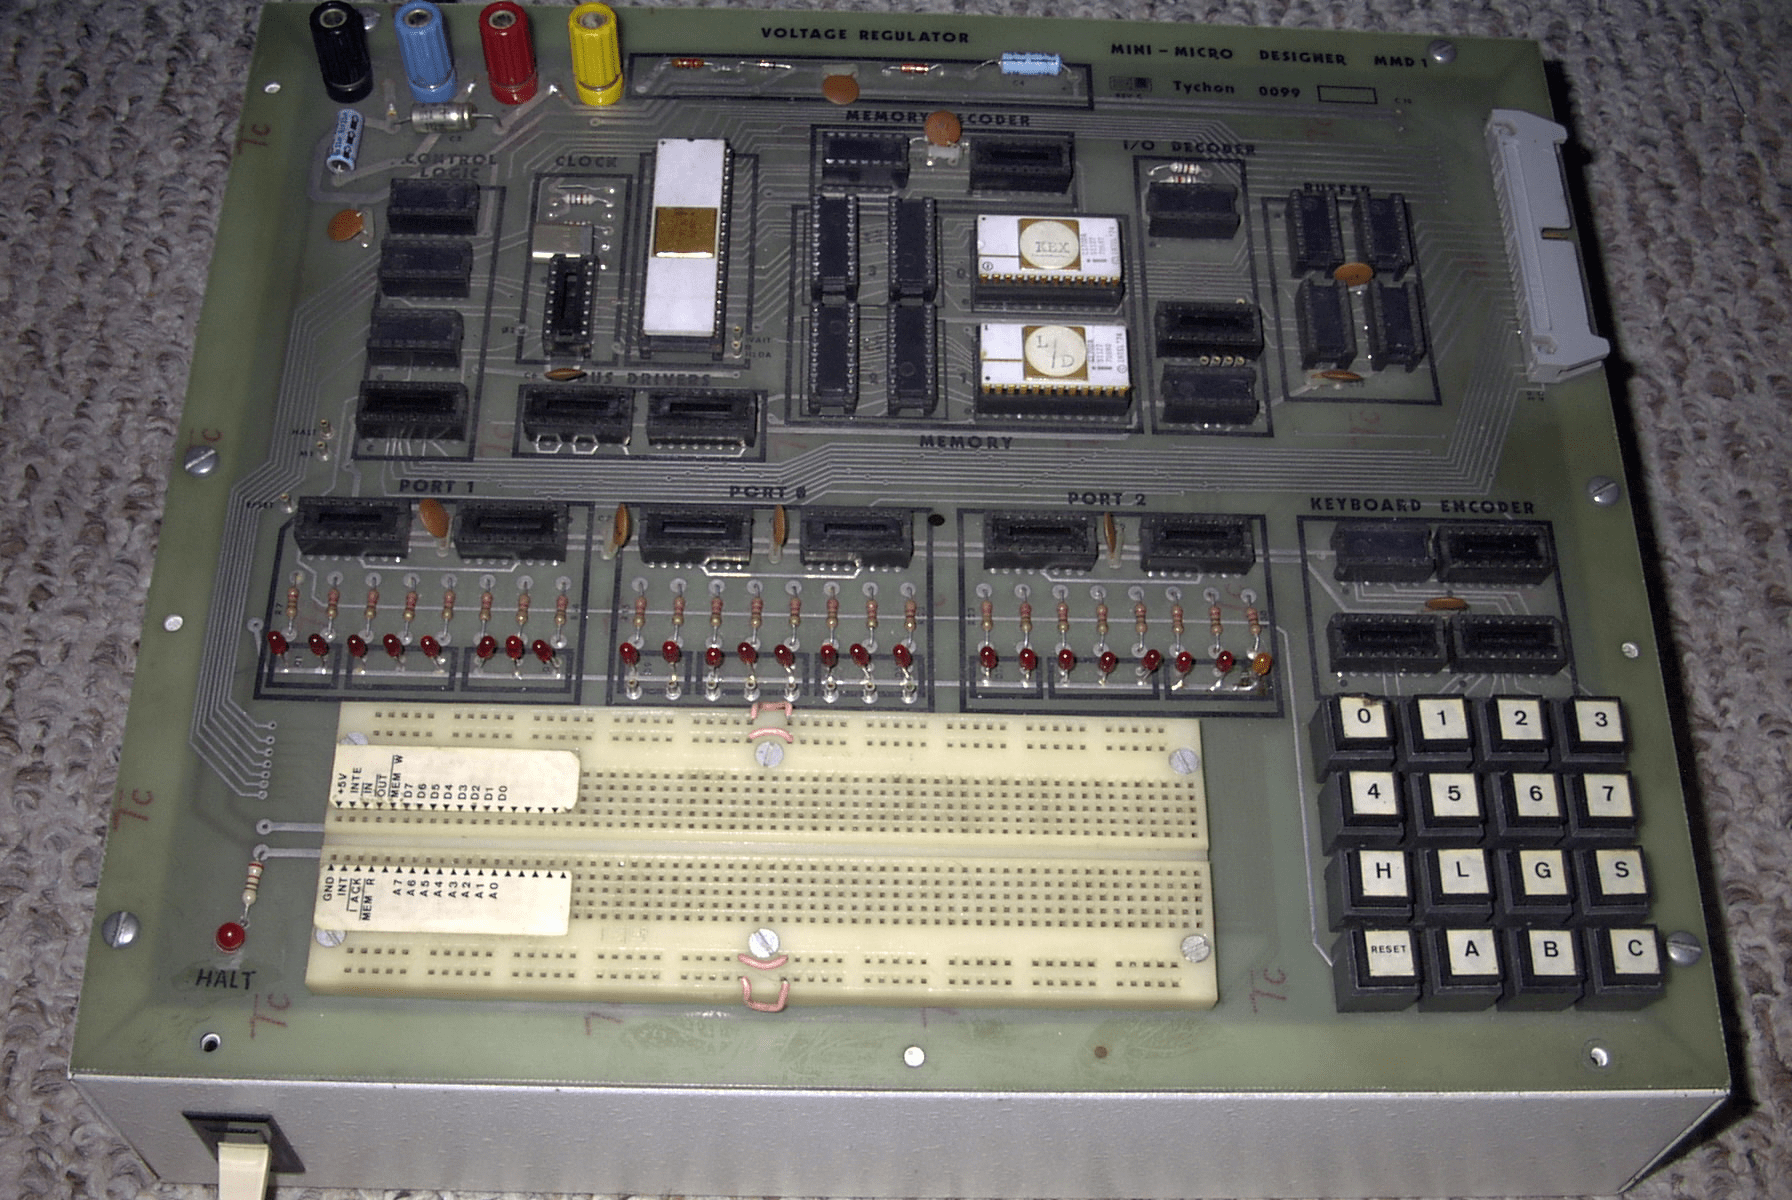
\includegraphics[width=120mm]{afbeeldingen/Early_1976_MMD1_Prototype_most_chips_removed.PNG}
		\caption{Eerste \gls{sbc}: MMD-1}
		\label{fig:eersteSBC}
	\end{figure}
	
	Naarmate dat de markt voor desktops en PC's groeide, nam de belangstelling voor \gls{sbc} in computers meer en meer af. Er werd verschoven naar een moederbord met de belangrijkste componenten en dochterborden voor periferiecomponenten zoals seriele poorten. De voornaamster reden hiervoor was dat de componenten groot waren. Alle onderdelen op dezelfde printplaat zou zorgen voor een onpraktisch ontwerp met grote afmetingen. Deze beweging was echter tijdelijk en naarmate de vorderende technologie kleinere componenten kon leveren, werden onderdelen terug naar het mainframe verschoven. Tegenwoordig kunnen de meeste moederborden terug als \gls{sbc} beschouwd worden. 

	
	In het jaar 2004 werd er in Itali\"e een nieuwe microcontroller uitgebracht onder de naam "Arduino". Dit ontwerp had naast het voordeel van compact en goedkoop te zijn, ook nog eenvoudigheid mee. Door de eenvoud werd het Arduino-platform snel populair onder techneuten van alle soorten. 
	Twee jaar later kwam er uit de Universiteit van Cambridge ook het nieuws van een nieuwe goedkope \gls{sbc} uit. De bekende Raspberry Pi werd gelanceerd voor de prijs van \$35. Het hoofddoel van dit project was een nieuw leermiddel om te programmeren maar werd door het grote aantal toepassingsmogelijkheden ook zeer populair.
	
	

%https://nl.wikipedia.org/wiki/Singleboardcomputer
\section{Benchmarking van \gls{ml} algoritmes}
\section{Assortiment aan 'on the shelf' toestellen}

	\subsection{Beaglebone AI}
	\subsection{Coral Dev }
	\subsection{Nvidia Jetson Nano}
	\subsection{Nvidia Jetson T2}
	\subsection{Raspberry Pi}
	\subsection{...}
	
	%specs van verschillende devices
	%waaromvraag beantwoorden, hoe lang nog supported

	

% waarom op de edge plaatsen van EBC (Voor en Nadelen) (miss meer situring)
% Specs van de verschillende boards 

%https://en.wikipedia.org/wiki/Artificial_neural_network
%https://en.wikipedia.org/wiki/Supervised_learning
%https://en.wikipedia.org/wiki/Unsupervised_learning
%https://en.wikipedia.org/wiki/Reinforcement_learning
%https://en.wikipedia.org/wiki/Artificial_neuron